\chapter{Relative Efficiency of Decoupled Adjoint Solver}
\label{chapter-nine}

At this point, the reacting gas adjoint in FUN3D has been utilized to obtain
sensitivity information needed to drive design optimization, and the
sensitivities of the fully coupled scheme have been validated against complex
Frechet derivatives for accuracy.  A key point of this study is to demonstrate
the increased computational efficiency and relative memory saving of using a
decoupled variable set for the flow and adjoint solvers, instead of a fully
coupled variable set.  This chapter details the benefits of applying the
decoupled adjoint solver over the fully coupled solver for the annular jet
demonstration problem.

\section{Verification of Consistency}
\label{adj-consistency}

Section \ref{block-jacobi-decoupling} showed in detail that, in the adjoint,
changing from the fully coupled variable and equation sets to the decoupled
variable and equation sets could be accomplished by a series of matrix
transformations on the Jacobian.  This transformation is equivalent to a left
and right preconditioning of the fully coupled scheme, enabling the reuse of the
approximate Jacobians used by the flow solver.  Provided the adjoint system is
well conditioned and convergence is sufficient, preconditioning should not
affect the final adjoint solution; thus, we expect to recover the exact same
solution from both the fully coupled and decoupled adjoint schemes.

The 5 $km/s$ spanwise cylinder case from \sref{sec:5-kps-cylinder} and the 15
$km/s$ sphere cone case from \sref{sec:15-kps-sphere-cone} are re-examined here
to determine the consistency of the adjoint solution computed by the fully
coupled schemes.  In this case, the sensitivity of the drag coefficient, $C_D$
to the angle of attack, $\alpha$, is computed by both schemes and compared.
%------------------------------------------------------------------------------%
\begin{table}[h]
  \centering
  \begin{tabular}{c|c|c|c}
    Case & Decoupled Sensitivity & Fully Coupled Sensitivity & Rel. Diff\\
    \hline
    Cylinder    &  0.764409218044021E-07 &  0.764409218054372E-07 & 1E-11 \\
    Sphere-Cone & -0.877773486565165E-02 & -0.877773486565157E-02 & 2E-14
  \end{tabular}
  \caption{Angle of attack sensitivity relative difference.}
  \label{tab:cylinder-adj-diff}
\end{table}
%------------------------------------------------------------------------------%
\tref{tab:cylinder-adj-diff} shows that the solutions match discretely to at
least 11 digits, and is indicative that the decoupled iterative mechanism can be
used to compute the adjoint solution without changing the result.  It should be
recognized here that, in the continuous sense, the drag on a cylinder is
independent of angle of attack; however, in the discrete sense of this grid,
which is only a half-body cylinder, there is a minimal dependence between angle
of attack and drag.

For the annular jet demonstration problem, the sensitivities computed in
\tref{tab:react-deriv-check} were checked to verify that decoupled and fully
coupled adjoint solutions matched to give the same sensitivity.
%------------------------------------------------------------------------------%
\begin{table}[h]
  \centering
  \begin{tabular}{c|c|c|c}
    Design Variable & Decoupled Sensitivity & Fully Coupled Sensitivity & Rel. Diff\\
    \hline
    $P_{p,o}$ & -0.11081315601976E-06 & -0.11081315649260E-06 & 4E-9  \\
    $T_{p,o}$ &  0.19089941243495E-03 &  0.19089941237390E-03 & 3E-10 \\
    $\fa$     & -0.28035409093945E-01 & -0.28035409045530E-01 & 1E-9
  \end{tabular}
  \caption{Annular jet plenum sensitivity relative difference.}
  \label{tab:srp-adj-diff}
\end{table}
%------------------------------------------------------------------------------%
\tref{tab:srp-adj-diff} also demonstrates excellent agreement between the
decoupled and fully coupled adjoint schemes.  Examining the differences of
sensitivities in \trefs{tab:cylinder-adj-diff}{tab:srp-adj-diff}, it is clear
that the absolute difference is almost always on the order of $10^{-15}$ for
each case.  Because double precision was used in all floating point operations for
these cases, these results are consistent with the level of precision used.

As a note on robustness, none of the stability issues found in the decoupled
flow solver have been observed for the decoupled adjoint scheme.  The
non-linear nature of the chemical source term was the primary stability concern
in the decoupled flow solver, because the explicitness introduced by the decoupled
mass fraction update exacerbates CFL restrictions.  These problems disappear in
the adjoint equations, because it is a linear system being solved instead of a
highly non-linear one.  The full stability and convergence properties of the
fully coupled adjoint solver were recovered by the decoupled adjoint solver, and
it is therefore concluded that there is no advantage of solving the adjoint
system in a fully coupled manner.

\section{Relative Memory Savings and Speedup}
\label{sec:adj-cost-mem-savings}

The computational cost of the solution process in the adjoint can be greatly
improved by storing the exact linearizations of the discrete flow solver
equations, as discussed in \sref{sec:2nd-order-mem-cost}.  For a second order
scheme 
%------------------------------------------------------------------------------%
\begin{figure}[h]
	\begin{subfigure}[b]{0.45\textwidth}
    \centering
    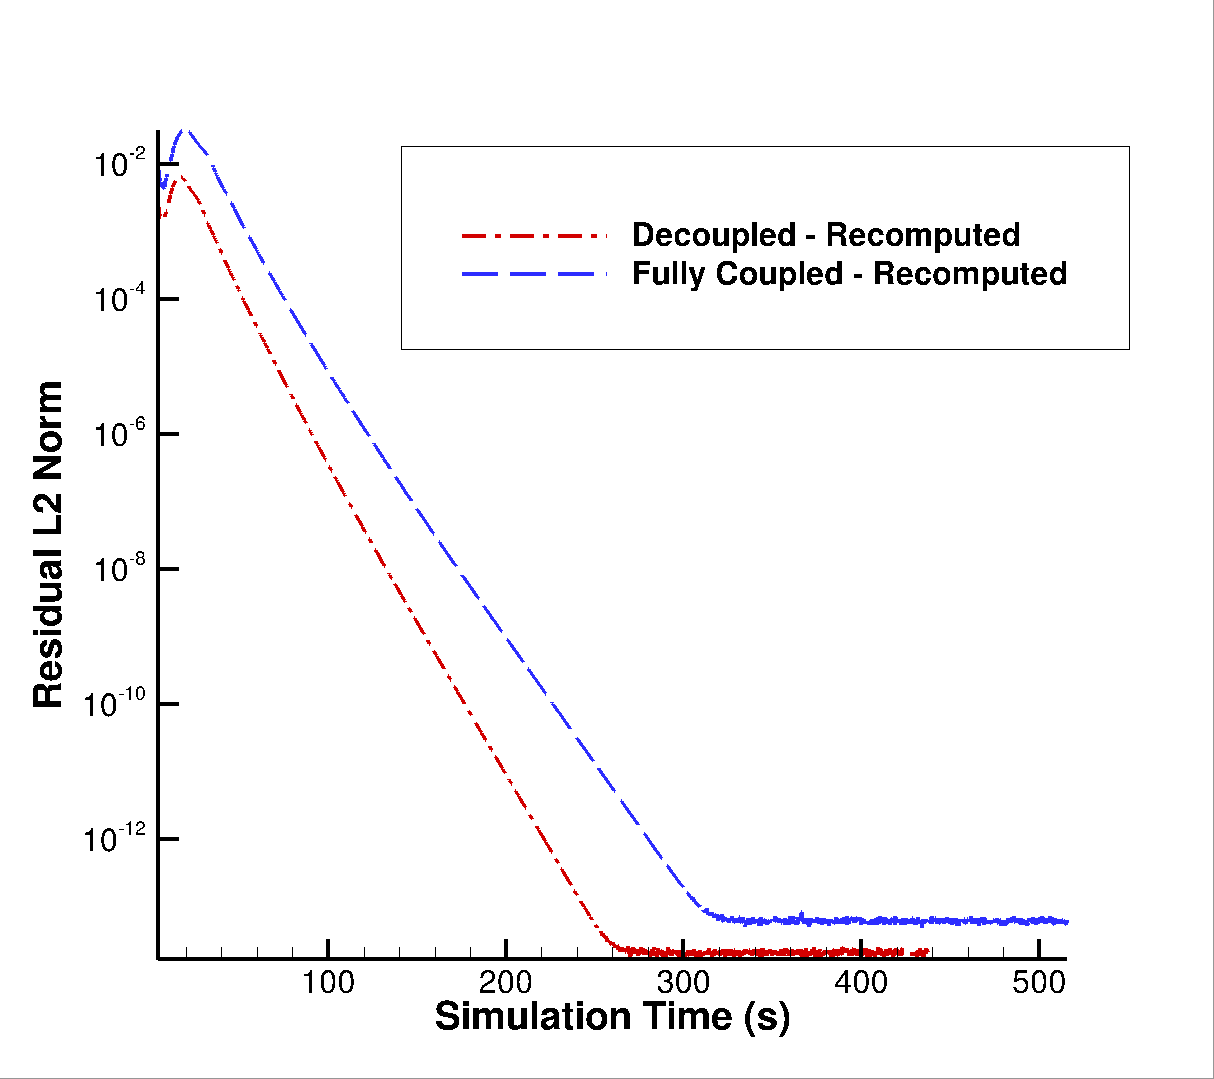
\includegraphics[width=\textwidth]{figures/adj-efficiency/adj-recompute.png}
    \caption{Linearizations always recomputed}
    \label{fig:always-recompute}
  \end{subfigure}
	\begin{subfigure}[b]{0.45\textwidth}
    \centering
    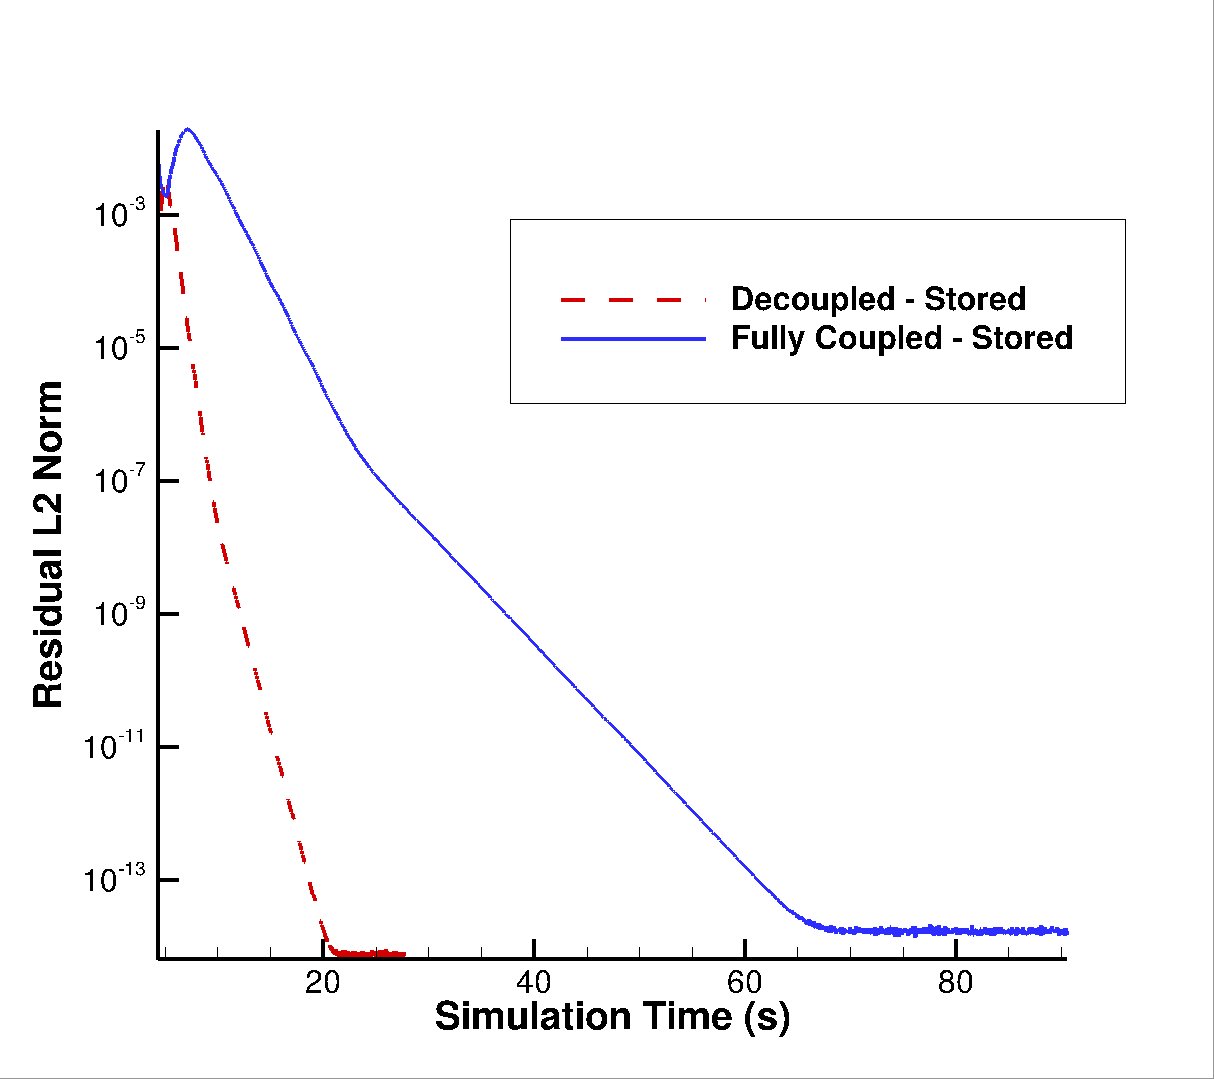
\includegraphics[width=\textwidth]{figures/adj-efficiency/adj-stored.png}
    \caption{Linearizations stored}
    \label{fig:stored}
  \end{subfigure}
  \caption{Simulation time comparison.}
  \label{fig:sim-time-comp}
\end{figure}
%------------------------------------------------------------------------------%
\fref{fig:sim-time-comp} shows the comparison of the fully coupled adjoint and 
decoupled adjoint time to solution with the two mechanisms for computing the
exact linearizations.  \tref{tab:srp-rel-speedup} shows that the reduction in
simulation time of the decoupled scheme is only truly realized when the exact
linearizations are stored, rather than recomputed at each timestep. 
%------------------------------------------------------------------------------%
\begin{table}[h]
  \centering
  \begin{tabular}{c|c|c|c}
    Scheme & Linearizations & Time to Convergence (s) & Speedup \\
    \hline
    Fully Coupled & Recomputed  & 309.4 & 1.0 (baseline)\\
    Decoupled     & Recomputed  & 244.2 & 1.27 \\
    Fully Coupled & Stored      & 61.22 & 5.05 \\
    Decoupled     & Stored      & 18.69 & $\mathbf{16.6}$ \\
  \end{tabular}
  \caption{Relative speedup.}
  \label{tab:srp-rel-speedup}
\end{table}
%------------------------------------------------------------------------------%
This reduction is because computing the exact linearizations in the adjoint is
the dominant cost.  The comparison between storing the linearizations and
recomputing them is somewhat unfair, as the ability to store the full Jacobian
of the second order reconstruction may not be possible, due to memory
constraints.  That said, a significant advantage of the decoupled scheme over
the fully coupled scheme is the memory savings offered by the LHS Jacobian
sparsity. It was show in \sref{sec:predicted-cost-mem-savings} that the
predicted memory savings for an infinite number of species is $1/7$ for a
hexahedra grid where the average number of neighbors is 6.  Unfortunately, the
storage requirements for the exact linearizations will not change between the
decoupled and fully coupled schemes; however, as the average number of neighbors
in the grid increases, the relative memory savings will also increase.  To
effectively demonstrate this, the amount of memory required by the adjoint
solver with the exact linearizations stored was determined for each mesh of the
refinement study in \sref{sec:mesh-refinement-study}.
%------------------------------------------------------------------------------%
\begin{figure}[h]
  \centering
	\begin{subfigure}[b]{0.45\textwidth}
    \centering
    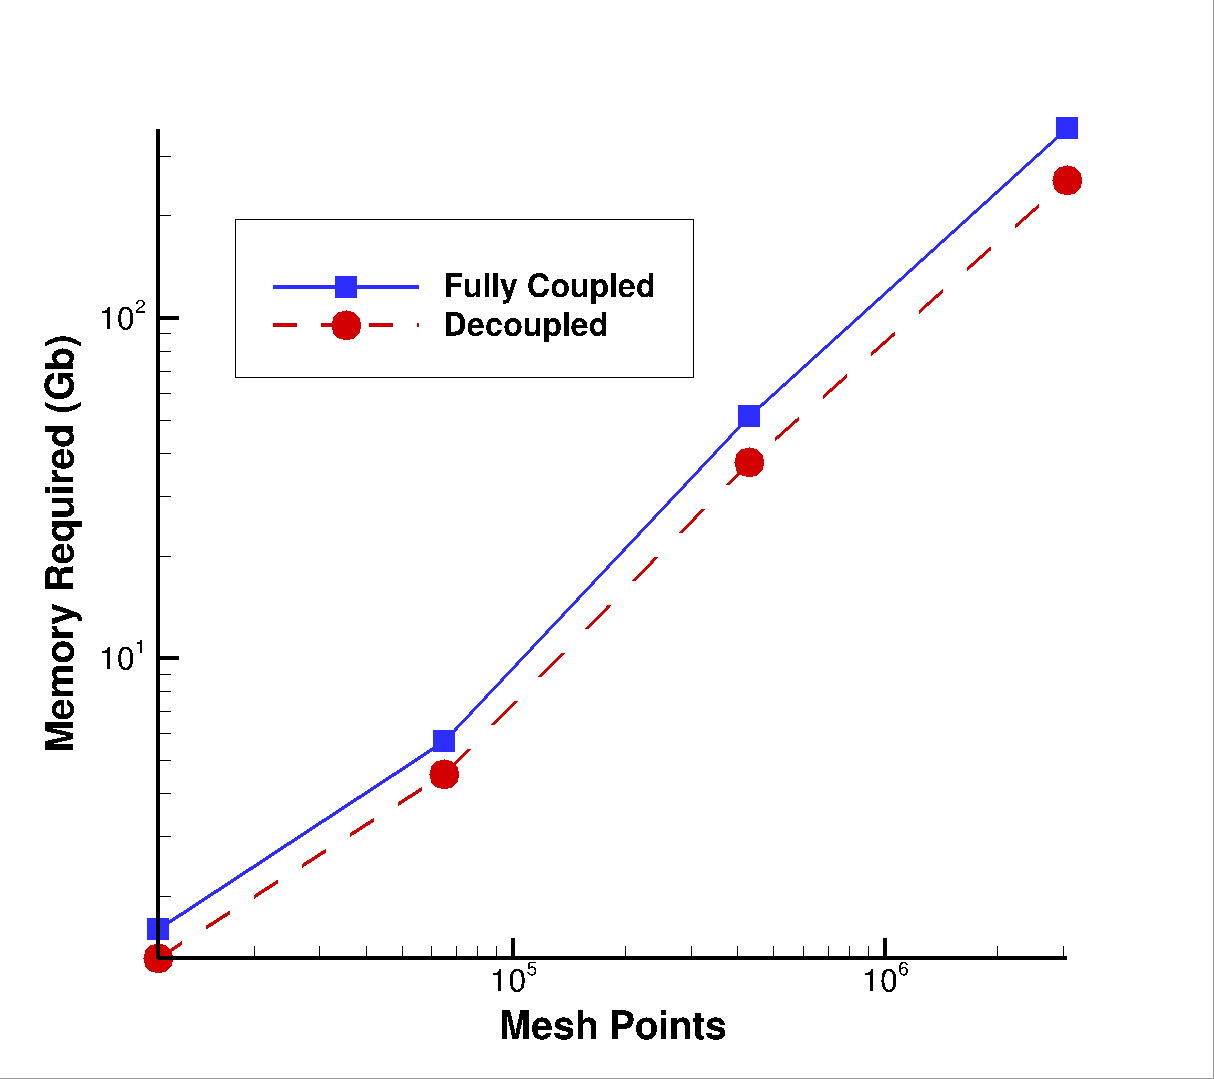
\includegraphics[width=\textwidth]{figures/adj-efficiency/mem-req-srp.png}
    \caption{Absolute memory required}
    \label{fig:abs-mem-req}
  \end{subfigure}
	\begin{subfigure}[b]{0.45\textwidth}
    \centering
    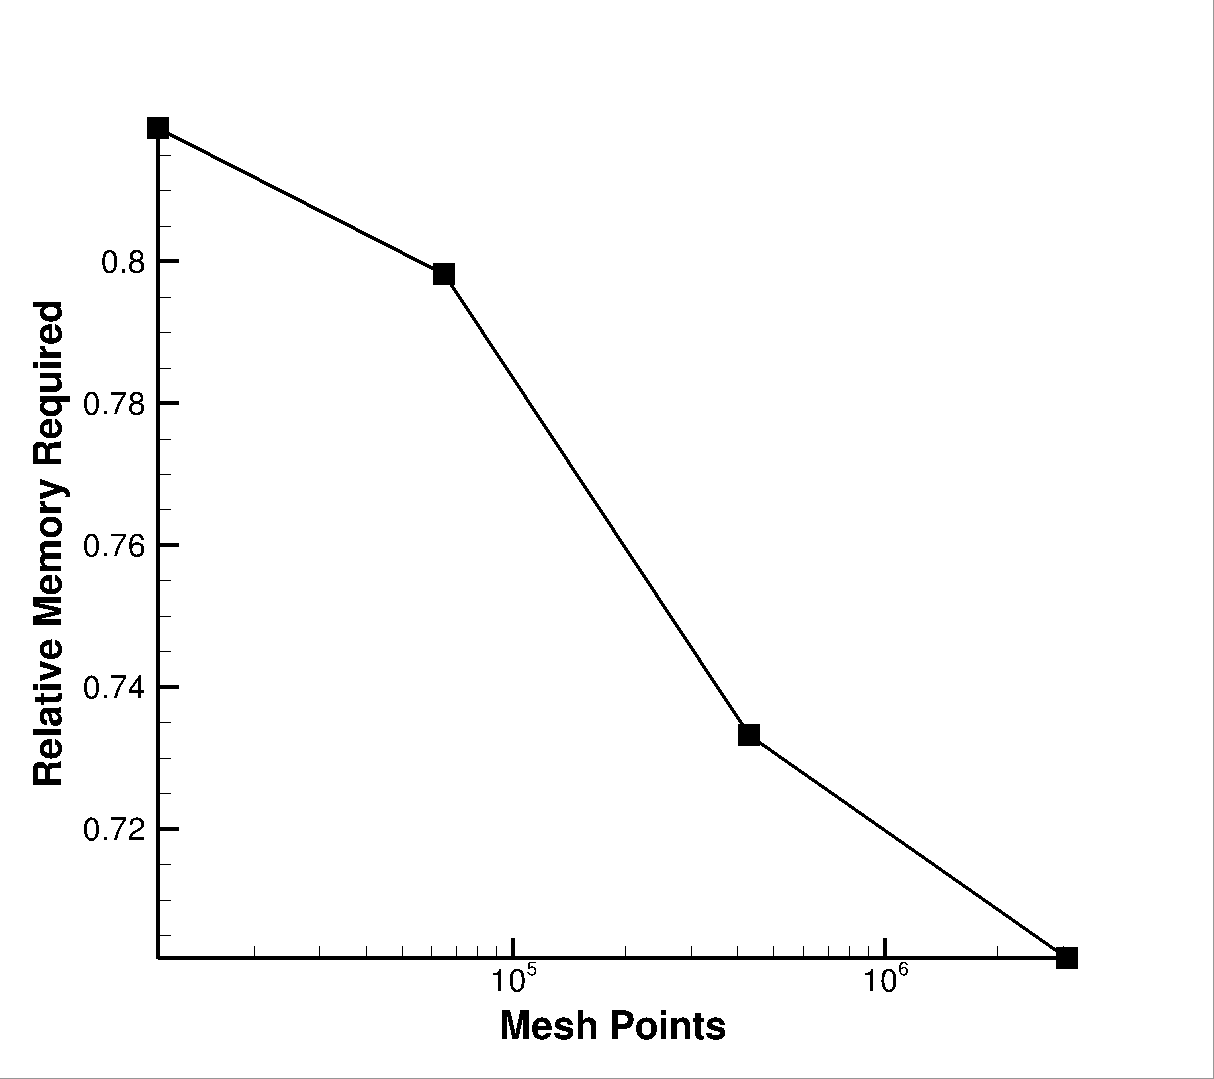
\includegraphics[width=\textwidth]{figures/adj-efficiency/mem-rel-savings.png}
    \caption{Relative memory required}
    \label{fig:relative-mem-req}
  \end{subfigure}
  \caption{Memory required to store full linearizations.}
  \label{fig:srp-mem-req}
\end{figure}
%------------------------------------------------------------------------------%
As shown in \fref{fig:srp-mem-req} it is possible to store the exact
linearizations for the 3.1 million node mesh, simulating a 9-species hydrogen
air mixture.  \fref{fig:abs-mem-req} show, as expected, that the memory
requirements for both the fully coupled and decoupled schemes scale directly
with the number of mesh points.  The relative savings for this case are nowhere
near the predicted $1/7$ value, because the exact linearizations require
significantly more memory than anything else in the adjoint solver.  That said,
the $\sim 20\%$ decrease in memory required by the decoupled adjoint solver is
significant, because the ability to store the exact linearizations is a binary
problem: either there is enough memory or there is not.  The increased savings
are as important as the reduction in simulation time, if not more so, because
the decoupled scheme can facilitate larger problems to be solved with greater
than an order of magnitude increase in computational efficiency, if the exact
linearizations can be stored.
